\section{Evaluation}
\label{sec:evaluation}

\definecolor{SpecBarBlue}{HTML}{6666FF}
\definecolor{SpecBarGreen}{HTML}{66BFBF}
\definecolor{SpecBarRed}{HTML}{FF6F6F}
\definecolor{SpecBarAmber}{HTML}{FFAD4D}
\definecolor{SpecBarTotal}{HTML}{8A8A8A}

We evaluate \tool{} on real protocol implementations and answer five research
questions:
\begin{itemize}[leftmargin=*]
  \item \textbf{RQ1: Field-centric rule discovery.} In a pooled open-world
  setting, how accurately and stably does \tool{} discover field-level rules
  for each protocol standard?
  \item \textbf{RQ2: Rule-to-code alignment.} How accurately does \tool{} map a
  standard rule to implementation variables and contexts?
  \item \textbf{RQ3: Bug finding.} In a pooled open-world setting, how many
  conformance-deviation reports does \tool{} discover, and how many are
  confirmed, fixed, rejected, pending, or assigned CVEs?
  \item \textbf{RQ4: Cost.} What is the LLM cost of generating submitted
  reports under GPT-5.4 pricing and across model providers?
  \item \textbf{RQ5: Ablation.} Which system components are responsible for the
  observed performance?
\end{itemize}

\subsection{Subjects and Baselines}

Table~\ref{tab:protocol-implementations} lists the evaluation subjects used in
this study. To ensure a fair comparison across different implementations, we
require \emph{all implementations of the same protocol version to share the same rule
set} extracted from the corresponding standard. For example, all TLS 1.3 
implementations are checked against the same 312 rules extracted from
RFC~8446~\cite{rfc8446}, and the two QUIC implementations are checked against
the same 286 rules extracted from RFC~9000~\cite{rfc9000}. Specifically, the
TLS/DTLS subjects include OpenSSL~\cite{openssl}, wolfSSL~\cite{wolfssl},
Mbed TLS~\cite{mbedtls}, openHiTLS, and BoringSSL~\cite{boringssl}; the QUIC
subjects include quiche~\cite{quiche} and ngtcp2~\cite{ngtcp2}; the MQTT
subjects include Mosquitto~\cite{mosquitto} and wolfMQTT~\cite{wolfmqtt}; and
the CoAP subject is libcoap~\cite{libcoap}.

\begin{table}[t]
\centering
\caption{Protocol implementations used for evaluation.}
\label{tab:protocol-implementations}
\resizebox{\columnwidth}{!}{
\setlength{\tabcolsep}{3pt}
\begin{tabular}{lcccl}
\toprule
\textbf{Subject} & \textbf{Version} & \textbf{LoC} & \textbf{Protocol} & \textbf{Specification} \\
\midrule
OpenSSL   & 11b7b6e & 1456.3K & TLS 1.3    & RFC 8446 \\
wolfSSL   & 1d363f3 & 520.4K  & TLS 1.3    & RFC 8446 \\
Mbed TLS  & 0fe989b & 310.8K  & TLS 1.3    & RFC 8446 \\
openHiTLS & 3d295814 & 480.2K & TLS 1.3    & RFC 8446 \\
Mosquitto & 99fa50f & 180.6K  & MQTT 5.0   & MQTT 5.0 \\
Mosquitto & 99fa50f & 180.6K  & MQTT 3.1.1 & MQTT 3.1.1 \\
wolfMQTT  & 88d37ed & 41.5K   & MQTT 3.1.1 & MQTT 3.1.1 \\
quiche    & 851533c & 92.3K   & QUIC       & RFC 9000 \\
ngtcp2    & 4af1c77 & 130.1K  & QUIC       & RFC 9000 \\
libcoap   & 7bc9a41 & 115.0K  & CoAP       & RFC 7252 \\
BoringSSL & 7f4d9a2 & 760.4K  & DTLS 1.3   & RFC 9147 \\
\bottomrule
\end{tabular}
}
\end{table}

We compare \tool{} against four baselines under the same subject versions,
rule budgets, model family, temperature setting, and maximum reasoning rounds.
\textbf{Direct Agent} receives the relevant standard section plus the top
keyword-retrieved code snippets and is asked to produce conformance reports
without field-space construction. \textbf{LLM+RAG} uses the same prompt schema
but retrieves code by embedding similarity over function-level chunks.
\textbf{Static-only} keeps \tool{}'s rule and code indexes but replaces LLM
semantic filtering and reasoning with deterministic alias, token-overlap, and
error-path heuristics. \textbf{w/o Test Agent} runs the full pipeline but does
not attempt executable validation. Each baseline uses the same top-15 file,
top-8 variable, top-12 snippet, and up to three evidence-completion rounds unless that
component is absent by design; prompt templates and raw outputs are included in
the artifact.

\subsection{Metrics and Ground Truth}

For rule extraction, we evaluate field-rule discovery in a pooled open-world
setting. To avoid bias toward any single LLM decoding run, we independently run
the full extractor three times for each extraction configuration. Candidate
rules from the three runs are first pooled and deduplicated by protocol
version, source span, constrained field, applicability condition, expected
action, and modality, forming the candidate pool for that configuration. 

We then compare the pool against the manually annotated benchmark of field-level
obligations. This benchmark was annotated by researchers from the TLS 1.3 and
MQTT 3.1.1 standards and contains 430 field-level obligations; each obligation
includes the source span, constrained field, condition, expected behavior, and
modality. If a candidate rule, after normalization, matches a gold obligation
in field, condition, action, and source semantics, it is counted as correctly
discovered. If a candidate rule matches no gold obligation, or corresponds to
unsupported normative text, erroneous splitting, or hallucinated requirements,
it is counted as a false discovery. If a gold obligation is not discovered in
any of the three runs for that configuration, it is counted as missed. The table 
values are therefore obtained by matching the pooled candidate rules against the 
430 gold obligations.

To evaluate code-context extraction, we use Var@1, Var@3, Ctx@1, Ctx@3, MRR,
and average token consumption. We stratify-sample 312 rule-implementation
pairs by protocol and implementation. Two authors with protocol and systems
experience independently annotate the correct implementation variable in each
sample and the minimal code context needed to determine the rule's behavior.
Disagreements are resolved by joint review of the standard span, callers,
validation helpers, and tests.

Here, Var@1 indicates whether the top-ranked candidate implementation variable
is the gold variable; Var@3 indicates whether the gold variable appears among
the top three candidates. Ctx@1 indicates whether the top-ranked code context
contains the key evidence required to judge the rule, such as a field
representation, a relevant check, error propagation, or an error-handling
path; Ctx@3 indicates whether at least one of the top three code contexts
contains such evidence. When evidence is spread across multiple functions, a
top-$k$ result is counted as a hit as long as the context bundle contains both
the decisive callee and caller. MRR measures the average position of the
correct result in the ranking list by taking the reciprocal rank of the first
correct candidate for each sample and averaging over all samples. For example,
a correct result at rank 1 scores 1, at rank 2 scores 1/2, and at rank 3
scores 1/3; if no correct result is found, the sample scores 0. Average token
consumption measures the number of LLM tokens consumed per rule-implementation
pair during alignment.

To evaluate the vulnerability-finding capability of different models, we conduct
a model-level comparison in a pooled open-world setting. Specifically, we run 
the full pipeline with four model families, namely GPT, Claude, DeepSeek, and 
Qwen, and repeat the experiment three times independently for each model. Candidate 
reports from all twelve runs are first pooled and deduplicated by protocol version, 
implementation, normative rule, and observed behavioral deviation, so that the same
issue is not counted multiple times. Security experts then manually adjudicate the 
deduplicated reports according to predefined correctness criteria and retain the true 
conformance deviations for each implementation. For a given model, a report is counted 
as discovered if the model finds it in at least one of its three runs. Based on this shared 
adjudicated report pool, we report the number of true reports and false positives discovered 
by each model, and define pooled coverage as the fraction of all adjudicated true reports 
found by that model. Pending reports are excluded from the precision denominator because 
their final status depends on maintainer response latency. Meanwhile, we do not claim that 
this metric represents whole-corpus recall.

A submitted report is a deduplicated candidate issue with a standard span, normalized rule, code evidence, and reproduction material when available. A confirmed fixed report is a submitted report that the maintainer fixed or explicitly confirmed as fixed. A false positive is a submitted report rejected by maintainer feedback or expert adjudication. A pending report has not yet received enough external signal for final adjudication. CVEs are counted only for previously unknown vulnerabilities assigned CVE identifiers after disclosure.

Our precision denominator is the adjudicated subset, not all submitted reports:
$\mathrm{P}_{adj}=\mathrm{Confirmed}/(\mathrm{Confirmed}+\mathrm{FP})$.

\subsection{RQ1: Field-Centric Rule Discovery}

Table~\ref{tab:field-rule-statistics} evaluates field-rule discovery on the manually
annotated TLS 1.3 and MQTT 3.1.1 benchmark. For each extraction configuration,
we independently run the extractor three times, then pool and deduplicate the
candidate rules from the three runs before matching them against the 430 gold
field-level obligations. We compare against three baselines: 0-shot prompt
directly extracts rules from the standard text; 2-shot prompt adds a few
examples to guide the model output; and Schema-only uses the same output schema
and validators as \tool{}, but does not construct a field space. All methods use
the same standard chunking and model settings.

\tool{} achieves the highest precision, coverage, and F1. The main reason is
that the field space provides clear protocol-object boundaries for rule
extraction. On the one hand, it reduces cases where descriptive text,
compatibility notes, or generic concepts are mistakenly extracted as field
rules. On the other hand, it helps the model resolve aliases, contextual
references, and cross-paragraph field constraints, thereby reducing missed
extractions. Therefore, \tool{}'s larger downstream rule set is not caused by
over-fragmenting standard text, but by more accurate discovery of field-level
obligations.

\begin{table}[t]
\centering
\caption{Field-rule discovery performance.}
\label{tab:field-rule-statistics}
\setlength{\tabcolsep}{3pt}
\begin{tabular}{lrrrrrrr}
\toprule
\textbf{Method} & \textbf{Extract.} & \textbf{TP} & \textbf{FP} & \textbf{FN}
& \textbf{Prec.} & \textbf{Cov.} & \textbf{F1} \\
\midrule
0-shot prompt  & 319 & 263 & 56 & 167 & 0.82 & 0.61 & 0.70 \\
2-shot prompt  & 384 & 323 & 61 & 107 & 0.84 & 0.75 & 0.79 \\
Schema-only   & 402 & 347 & 55 & 83  & 0.86 & 0.81 & 0.83 \\
\tool{}       & 439 & 407 & 32 & 23  & 0.93 & 0.95 & 0.94 \\
\bottomrule
\end{tabular}
\end{table}

\subsection{RQ2: Rule-to-Code Alignment}

Table~\ref{tab:alignment} shows that field-aware localization substantially
improves rule-to-code alignment. Compared with Exact Match, BM25, Embedding,
and LLM Direct, \tool{} achieves the best overall performance in both variable
recovery and context recovery. Exact Match relies on lexical overlap, BM25 uses
sparse lexical retrieval, Embedding uses dense semantic retrieval, and LLM
Direct feeds retrieved code directly to the LLM without field-aware
localization.

\tool{} achieves 0.79 Var@1 and 0.91 Var@3, indicating that the correct
implementation variable is usually ranked near the top. It also achieves 0.74
Ctx@1 and 0.87 Ctx@3, showing that the retrieved contexts more often contain
the decisive evidence needed for checking a rule, such as validation logic,
error propagation, or state updates. This improvement is important because many
false positives arise when retrieval returns nearby but semantically irrelevant
functions. Meanwhile, \tool{} consumes 5.2K tokens on average, compared with
7.1K tokens for LLM Direct, suggesting that field-aware localization improves
alignment quality while keeping the evidence bundle more compact.

\begin{table}[t]
\centering
\caption{Effectiveness of rule-to-code alignment.}
\label{tab:alignment}
\resizebox{\columnwidth}{!}{
\setlength{\tabcolsep}{3pt}
\begin{tabular}{lrrrrrr}
\toprule
\textbf{Method} & \textbf{Var@1} & \textbf{Var@3} & \textbf{Ctx@1} & \textbf{Ctx@3} & \textbf{MRR} & \textbf{Tok.} \\
\midrule
Exact Match & 0.34 & 0.48 & 0.29 & 0.43 & 0.41 & 0.9K \\
BM25 & 0.41 & 0.56 & 0.36 & 0.51 & 0.48 & 1.3K \\
Embedding & 0.47 & 0.64 & 0.43 & 0.59 & 0.55 & 2.5K \\
LLM Direct & 0.72 & 0.84 & 0.69 & 0.88 & 0.78 & 7.1K \\
\tool{} & 0.79 & 0.91 & 0.74 & 0.87 & 0.84 & 5.2K \\
\bottomrule
\end{tabular}
}
\end{table}

\paragraph{Context-retrieval prior ablation.}
The coefficients in Equation~(1) are fixed retrieval priors rather than
project-specific learned weights. Table~\ref{tab:sensitivity} ablates the
retrieval signals and varies their weights to test whether Equation~(1) depends
on fragile constants. Here, variable-token overlap means the overlap between a
candidate snippet and tokens from the localized implementation variable; rule-token
overlap means the overlap between a candidate snippet and tokens from the
field-level rule; and the action-role bonus $b(c)$ rewards snippets where the
candidate field participates in validation, comparison, assignment, error
handling, or state updates. The results show that removing exact-field matches
causes the largest performance drop, while removing weaker terms leads to more
gradual degradation in alignment quality. When the exact-field, variable-token,
and rule-token weights are scaled within a factor of two while preserving their
relative order, the alignment metrics remain stable. In contrast, the largest
degradation appears when the retrieval-signal hierarchy is broken, especially
when exact-field matches are removed, $b(c)$ is disabled, or all weights are
assigned uniform values. These results suggest that \tool{}'s alignment quality
mainly comes from the retrieval-signal hierarchy and syntax-aware features,
rather than from a narrowly tuned set of constants. In Table~\ref{tab:sensitivity},
``var. tok.'' and ``rule tok.'' denote variable-token and rule-token overlap,
respectively.



\begin{table}[t]
\centering
\caption{Sensitivity of rule-to-code alignment signals.}
\label{tab:sensitivity}
\resizebox{\columnwidth}{!}{
\setlength{\tabcolsep}{3pt}
\begin{tabular}{lcccrrr}
\toprule
\textbf{Setting} & \textbf{$w_{\mathrm{exact}}$} & \textbf{$w_{\mathrm{var}}$} & \textbf{$w_{\mathrm{rule}}$} & \textbf{Var@1} & \textbf{Ctx@1} & \textbf{MRR} \\
\midrule
Default                         & 5.0  & 0.90 & 0.28 & 0.79 & 0.74 & 0.84 \\
No exact                        & 0.0  & 0.90 & 0.28 & 0.70 & 0.63 & 0.75 \\
No var. tok.                    & 5.0  & 0.00 & 0.28 & 0.73 & 0.66 & 0.78 \\
No rule tok.                    & 5.0  & 0.90 & 0.00 & 0.77 & 0.72 & 0.82 \\
No action                       & 5.0  & 0.90 & 0.28 & 0.75 & 0.69 & 0.80 \\
$w_{\mathrm{exact}}\times 0.5$ & 2.5  & 0.90 & 0.28 & 0.78 & 0.73 & 0.83 \\
$w_{\mathrm{exact}}\times 2$   & 10.0 & 0.90 & 0.28 & 0.79 & 0.74 & 0.84 \\
$w_{\mathrm{var}}\times 0.5$   & 5.0  & 0.45 & 0.28 & 0.78 & 0.73 & 0.83 \\
$w_{\mathrm{var}}\times 2$     & 5.0  & 1.80 & 0.28 & 0.79 & 0.74 & 0.84 \\
$w_{\mathrm{rule}}\times 0.5$  & 5.0  & 0.90 & 0.14 & 0.78 & 0.73 & 0.83 \\
$w_{\mathrm{rule}}\times 2$    & 5.0  & 0.90 & 0.56 & 0.78 & 0.73 & 0.83 \\
Uniform weights                 & 1.0  & 1.00 & 1.00 & 0.74 & 0.68 & 0.79 \\
\bottomrule
\end{tabular}
}
\end{table}


\subsection{RQ3: Bug Finding Results}

\begin{table}[t]
\centering
\caption{Status of submitted conformance-deviation reports and maintainer outcomes.
\#R denotes the number of rules used for each protocol version. 
Sub. is the number of reports submitted to maintainers, 
Conf. is the number of reports confirmed or fixed by maintainers, 
FP is the number of rejected false positives, 
and Pend. is the number of reports still awaiting final maintainer response.}
\label{tab:verification-results}
\normalsize
\setlength{\tabcolsep}{3pt}
\begin{tabular}{llrrrrr}
\toprule
\textbf{Subject}
& \textbf{Protocol}
& \textbf{\#R}
& \textbf{Sub.}
& \textbf{Conf.}
& \textbf{FP}
& \textbf{Pend.} \\
\midrule
OpenSSL    & TLS 1.3    & 312 & 14 & 9  & 1 & 4 \\
wolfSSL    & TLS 1.3    & 312 & 23 & 15 & 1 & 7 \\
Mbed TLS   & TLS 1.3    & 312 & 17 & 11 & 1 & 5 \\
openHiTLS  & TLS 1.3    & 312 & 19 & 12 & 1 & 6 \\
Mosquitto  & MQTT 5.0   & 164 & 21 & 13 & 1 & 7 \\
Mosquitto  & MQTT 3.1.1 & 127 & 16 & 10 & 0 & 6 \\
wolfMQTT   & MQTT 3.1.1 & 127 & 22 & 14 & 1 & 7 \\
quiche     & QUIC       & 286 & 24 & 15 & 1 & 8 \\
ngtcp2     & QUIC       & 286 & 18 & 11 & 1 & 6 \\
libcoap    & CoAP       & 143 & 18 & 11 & 1 & 6 \\
BoringSSL  & DTLS 1.3   & 198 & 12 & 5  & 0 & 7 \\
\midrule
Total      & --         & --  & 204 & 126 & 9 & 69 \\
\bottomrule
\end{tabular}
\end{table}

Table~\ref{tab:verification-results} summarizes the status of reports that were
submitted to repository maintainers. The table does not count all intermediate
candidate findings produced by the pipeline. Instead, it reports the final
deduplicated submissions and their maintainer outcomes. In total, \tool{}
submitted 204 conformance-deviation reports. Maintainers have confirmed or fixed
126 of them, rejected 9 as false positives, and 69 remain pending. Two confirmed
reports correspond to previously unknown vulnerabilities and were assigned CVE
identifiers after disclosure. 

% We therefore treat maintainer-confirmed fixes and
% assigned CVEs as strong external evidence, while pending reports are not counted
% as confirmed bugs.

\begin{table*}[t]
\centering
\caption{Per-model comparison on conformance inconsistency detection in the
pooled open-world setting. The twelve runs are pooled and deduplicated by
protocol version, implementation, normative rule, and observed behavioral
deviation. Adj.P excludes pending reports from the denominator.}
\label{tab:llm-comparison-implementation-full}
\resizebox{\textwidth}{!}{
\normalsize
\setlength{\tabcolsep}{3pt}
\begin{tabular}{lr|rrrr|rrrr|rrrr|rrrr|c}
\toprule
\textbf{Protocol}
& \textbf{\#R}
& \multicolumn{4}{c|}{\textbf{GPT-5.4}}
& \multicolumn{4}{c|}{\textbf{DeepSeek}}
& \multicolumn{4}{c|}{\textbf{Claude}}
& \multicolumn{4}{c|}{\textbf{Qwen}}
& \textbf{Avg. Adj.P} \\
\cmidrule(lr){3-6}
\cmidrule(lr){7-10}
\cmidrule(lr){11-14}
\cmidrule(lr){15-18}
& & \textbf{Sub.} & \textbf{Conf.} & \textbf{FP} & \textbf{Adj.P}
& \textbf{Sub.} & \textbf{Conf.} & \textbf{FP} & \textbf{Adj.P}
& \textbf{Sub.} & \textbf{Conf.} & \textbf{FP} & \textbf{Adj.P}
& \textbf{Sub.} & \textbf{Conf.} & \textbf{FP} & \textbf{Adj.P}
& \\
\midrule
TLS 1.3
& 312
& 73 & 47 & 4 & 0.92
& 62 & 37 & 7 & 0.84
& 68 & 42 & 6 & 0.88
& 56 & 31 & 7 & 0.82
& 0.86 \\
QUIC
& 286
& 42 & 26 & 2 & 0.93
& 36 & 21 & 4 & 0.84
& 39 & 24 & 4 & 0.86
& 33 & 18 & 4 & 0.82
& 0.86 \\
MQTT 5.0
& 164
& 21 & 13 & 1 & 0.93
& 18 & 10 & 2 & 0.83
& 19 & 12 & 2 & 0.86
& 17 & 9 & 2 & 0.82
& 0.86 \\
MQTT 3.1.1
& 127
& 38 & 24 & 1 & 0.96
& 32 & 19 & 3 & 0.86
& 34 & 21 & 3 & 0.88
& 28 & 16 & 4 & 0.80
& 0.88 \\
CoAP
& 143
& 18 & 11 & 1 & 0.92
& 16 & 10 & 1 & 0.91
& 17 & 10 & 2 & 0.83
& 15 & 9 & 2 & 0.82
& 0.87 \\
DTLS 1.3
& 198
& 12 & 5 & 0 & 1.00
& 12 & 5 & 1 & 0.83
& 11 & 5 & 2 & 0.71
& 10 & 4 & 2 & 0.67
& 0.80 \\
\midrule
Total
& 1230
& 204 & 126 & 9  & -
& 176 & 102 & 18 & -
& 188 & 114 & 19 & -
& 159 & 87  & 21 & -
& - \\
\bottomrule
\end{tabular}
}
\end{table*}

% \begin{figure}[t]
% \centering
% \begin{tikzpicture}
% \begin{axis}[
%   ybar,
%   width=\columnwidth,
%   height=4.7cm,
%   ymin=0,
%   ymax=220,
%   ylabel={Reports},
%   xmin=-0.38,
%   xmax=2.42,
%   xtick={0,0.68,1.36,2.04},
%   xticklabels={GPT-5.4,DeepSeek,Claude,Qwen},
%   x tick label style={font=\scriptsize},
%   tick label style={font=\scriptsize},
%   label style={font=\scriptsize},
%   legend style={at={(0.5,1.04)}, anchor=south, legend columns=2,
%     draw=none, font=\scriptsize, /tikz/every even column/.append style={column sep=2pt}},
%   bar width=6.4pt,
%   enlarge x limits=false,
%   ymajorgrids=true,
%   grid style={gray!20},
% ]
% \addplot[fill=SpecBarBlue, draw=SpecBarBlue!70!black, bar shift=-9.6pt] coordinates {
%   (0,204) (0.68,176) (1.36,188) (2.04,159)
% };
% \addplot[fill=SpecBarGreen, draw=SpecBarGreen!70!black, bar shift=-3.2pt] coordinates {
%   (0,126) (0.68,102) (1.36,114) (2.04,87)
% };
% \addplot[fill=SpecBarRed, draw=SpecBarRed!70!black, bar shift=3.2pt] coordinates {
%   (0,9) (0.68,18) (1.36,19) (2.04,21)
% };
% \addplot[fill=SpecBarAmber, draw=SpecBarAmber!70!black, bar shift=9.6pt] coordinates {
%   (0,69) (0.68,56) (1.36,55) (2.04,51)
% };
% \legend{Submitted, Confirmed/fixed, False positive, Pending}
% \end{axis}
% \end{tikzpicture}
% \caption{Aggregate report status by model. The figure summarizes
% Table~\ref{tab:llm-comparison-implementation-full} across all evaluated
% protocols while keeping the same non-model components fixed.}
% \label{fig:model-comparison-bars}
% \end{figure}

% To evaluate the bug-finding capability of different model families,
% Table~\ref{tab:llm-comparison-implementation-full} and
% Figure~\ref{fig:model-comparison-bars} compare their report outcomes under the
% same pipeline setting. We fix all non-model components to ensure a fair
% comparison across models. Specifically, each model uses the same extracted
% rules, code-retrieval budget, validators, adjudication protocol, and test-agent
% settings. The code-retrieval budget includes the number of candidate files,
% candidate variables, and code snippets that can be retrieved for each rule, as
% well as the maximum number of evidence-completion rounds. Therefore, different
% models are given rule sets and code evidence of the same scale, and the
% differences mainly come from the models' semantic understanding, code reasoning,
% and report-generation capabilities. Prompt differences are limited to
% model-specific formatting constraints needed to obtain schema-valid JSON
% outputs. The results show that GPT-5.4 produces the largest number of
% maintainer-confirmed fixes. In contrast, smaller or less code-specialized models
% produce more false-positive reports. Provider-level cost differences are
% analyzed separately in RQ4.

To evaluate the bug-finding capability of different model families,
Table~\ref{tab:llm-comparison-implementation-full} compare their report outcomes under the
same pipeline setting. We fix all non-model components to ensure a fair
comparison across models. Specifically, each model uses the same extracted
rules, code-retrieval budget, validators, adjudication protocol, and test-agent
settings. The code-retrieval budget includes the number of candidate files,
candidate variables, and code snippets that can be retrieved for each rule, as
well as the maximum number of evidence-completion rounds. Therefore, different
models are given rule sets and code evidence of the same scale, and the
differences mainly come from the models' semantic understanding, code reasoning,
and report-generation capabilities. Prompt differences are limited to
model-specific formatting constraints needed to obtain schema-valid JSON
outputs. The results show that GPT-5.4 produces the largest number of
maintainer-confirmed fixes. In contrast, smaller or less code-specialized models
produce more false-positive reports. Provider-level cost differences are
analyzed separately in RQ4.


%运行稳定性
% \paragraph{Run-to-run stability.}
% Because \tool{} uses LLMs in extraction, filtering, reasoning, and test
% planning, we reran the full GPT-5.4 pipeline three times with independent
% decoding seeds and empty caches for the LLM stages. Table~\ref{tab:stability}
% reports mean and standard deviation over the repeated runs.

% \begin{table}[t]
% \centering
% \caption{Run-to-run stability over three GPT-5.4 runs.}
% \label{tab:stability}
% \small
% \begin{tabular}{lrr}
% \toprule
% \textbf{Metric} & \textbf{Mean} & \textbf{Std. dev.} \\
% \midrule
% Submitted reports & 202.7 & 5.9 \\
% Confirmed/fixed reports & 124.3 & 4.7 \\
% False positives & 10.3 & 2.5 \\
% Pending reports & 68.0 & 3.6 \\
% Adj.P & 0.92 & 0.02 \\
% \bottomrule
% \end{tabular}
% \end{table}

\FloatBarrier

\subsection{RQ4: Cost Analysis}

To evaluate the model cost of \tool{}, we use GPT-5.4 pricing as the cost
model. Table~\ref{tab:cost} breaks down the average cost per report by pipeline
stage, including rule extraction, code-context extraction, consistency
reasoning, and the verification-test agent. The largest cost comes from consistency reasoning, which costs \$0.431 per
report on average and accounts for 38.4\% of the total cost. This is because a
suspicious finding usually cannot be judged in a single round. Instead, it often
requires multiple evidence-completion rounds, such as retrieving callers, macro
definitions, error-propagation paths, or configuration branches. Code-context
extraction is the second-largest cost component, accounting for 25.3\%, because
the system needs to semantically filter candidate files, variables, and code
snippets before reasoning. The verification-test agent accounts for 20.6\%,
mainly due to test-plan generation, harness adaptation, and log interpretation.
In contrast, rule extraction accounts for only 15.7\%, because the rule set for
the same protocol version can be reused across multiple implementations and its
cost is therefore amortized.

Figure~\ref{fig:model-cost-bars} further compares the same stage-wise cost
breakdown across the four model families used in
Table~\ref{tab:llm-comparison-implementation-full}. Claude has the highest
estimated total cost, followed by GPT-5.4, while DeepSeek and Qwen are about
35\% cheaper than GPT-5.4. These results show a trade-off between model cost and
bug-finding capability: lower-cost models reduce analysis expense, but, as shown
above, they generally produce fewer maintainer-confirmed fixes or more false
positives. In practice, one possible deployment strategy is to use lower-cost
models for initial screening and then use stronger models to recheck high-risk
rules or suspicious reports.

\begin{table}[t]
\centering
\caption{Average GPT-5.4 model cost per submitted report.}
\label{tab:cost}
\small
\begin{tabular}{lrr}
\toprule
\textbf{Stage} & \textbf{Cost / Report} & \textbf{Share} \\
\midrule
Rule extraction & \$0.176 & 15.7\% \\
Code-context extraction & \$0.284 & 25.3\% \\
Consistency reasoning & \$0.431 & 38.4\% \\
Verification-test agent & \$0.231 & 20.6\% \\
\midrule
Total & \$1.122 & 100.0\% \\
\bottomrule
\end{tabular}
\end{table}

\begin{figure}[!t]
\centering
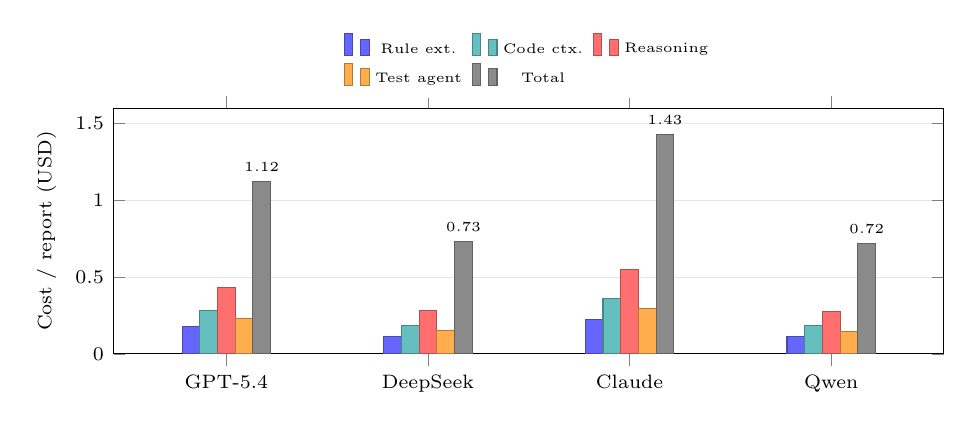
\begin{tikzpicture}
\begin{axis}[
  ybar,
  width=\columnwidth,
  height=4.7cm,
  ymin=0,
  ymax=1.6,
  ylabel={Cost / report (USD)},
  xmin=-0.38,
  xmax=2.42,
  xtick={0,0.68,1.36,2.04},
  xticklabels={GPT-5.4,DeepSeek,Claude,Qwen},
  x tick label style={font=\scriptsize},
  tick label style={font=\scriptsize},
  label style={font=\scriptsize},
  legend style={at={(0.5,1.04)}, anchor=south, legend columns=3,
    draw=none, font=\tiny, /tikz/every even column/.append style={column sep=1.5pt}},
  bar width=6.4pt,
  enlarge x limits=false,
  ymajorgrids=true,
  grid style={gray!20},
]
\addplot[fill=SpecBarBlue, draw=SpecBarBlue!70!black, bar shift=-12.8pt] coordinates {
  (0,0.176) (0.68,0.115) (1.36,0.225) (2.04,0.113)
};
\addplot[fill=SpecBarGreen, draw=SpecBarGreen!70!black, bar shift=-6.4pt] coordinates {
  (0,0.284) (0.68,0.185) (1.36,0.362) (2.04,0.182)
};
\addplot[fill=SpecBarRed, draw=SpecBarRed!70!black, bar shift=0pt] coordinates {
  (0,0.431) (0.68,0.280) (1.36,0.549) (2.04,0.276)
};
\addplot[fill=SpecBarAmber, draw=SpecBarAmber!70!black, bar shift=6.4pt] coordinates {
  (0,0.231) (0.68,0.150) (1.36,0.295) (2.04,0.148)
};
\addplot[fill=SpecBarTotal, draw=SpecBarTotal!70!black, bar shift=12.8pt,
  nodes near coords={\pgfmathprintnumber[fixed,precision=2]{\pgfplotspointmeta}},
  nodes near coords style={font=\tiny, /pgf/number format/fixed}] coordinates {
  (0,1.122) (0.68,0.73) (1.36,1.43) (2.04,0.72)
};
\legend{Rule ext., Code ctx., Reasoning, Test agent, Total}
\end{axis}
\end{tikzpicture}
\caption{Average model cost per submitted report by model family and pipeline
stage. The GPT-5.4 bars correspond to Table~\ref{tab:cost}}
\label{fig:model-cost-bars}
\end{figure}

\subsection{RQ5: Ablation Study}

Taking GPT-5.4 as the example, Table~\ref{tab:ablation} shows how different
system components affect discovery capability and result quality. Direct Agent
and LLM+RAG cover 70.1\% and 64.7\% of the reports, respectively, showing that
standard snippets and generic code retrieval alone do not reliably obtain the
implementation evidence needed for rule checking. In contrast, Static-only
keeps the rule representation and code indexes, increasing coverage to 83.3\%.
This result indicates that field-space construction and field-level code
localization substantially expand the discoverable range. However, Static-only
replaces LLM semantic filtering and reasoning with deterministic alias matching,
token overlap, and error-path heuristics. Its false positives therefore rise to
78 and its adjusted precision drops to 0.60, showing that field localization
helps the system find more potential evidence but is still insufficient for
renamed fields, cross-function checks, and indirect error propagation.

Removing iterative reasoning reduces coverage to 78.9\%. This result shows that
the \textsc{Insufficient} state and the evidence completion it triggers are not
only a conservative way to record uncertainty, but also directly affect
discovery capability. When the current evidence lacks callers, macro
definitions, validation helpers, or error-propagation paths, the system must
continue retrieving and completing context before a potential deviation can be
submitted as a report. The Forced-binary result further supports this point:
forcing low-evidence samples into either consistent or inconsistent verdicts
covers only 85.8\% of the reports and increases false positives to 63, showing
that explicitly preserving \textsc{Insufficient} is more reliable than premature
binary adjudication. Without the test agent, the system still reaches 93.1\%
coverage, but false positives increase to 33, indicating that runtime
validation mainly filters and confirms high-risk reports rather than simply
increasing the number of candidates. The full system combines field-space
construction, semantic reasoning, \textsc{Insufficient}-driven evidence
completion, and test validation, reaching the highest coverage of 95.6\% while
maintaining an adjusted precision of 0.87.


\begin{table}[t]
\centering
\caption{Ablation results on the adjudicated report set. Cov. denotes the
percentage of the 204 reports discovered by each variant, not whole-corpus
recall.}
\label{tab:ablation}
\small
\setlength{\tabcolsep}{4pt}
\begin{tabular}{lrrrrrc}
\toprule
\textbf{Configuration}
& \textbf{Sub.}
& \textbf{Conf.}
& \textbf{FP}
& \textbf{Pend.}
& \textbf{Adj.P}
& \textbf{Cov. (\%)} \\
\midrule
Direct Agent
& 143 & 72  & 24 & 47 & 0.75 & 70.1 \\

LLM+RAG
& 132 & 73  & 9  & 50 & 0.89 & 64.7 \\

Static-only
& 170 & 116 & 78 & 54 & 0.60 & 83.3 \\

w/o Ite Rea
& 161 & 101 & 15 & 60 & 0.87 & 78.9 \\

w/o Test Agent
& 190 & 126 & 33 & 64 & 0.79 & 93.1 \\

Forced binary
& 175 & 111 & 63 & 64 & 0.64 & 85.8 \\

Full System
& 195 & 126 & 19 & 69 & 0.87 & 95.6 \\
\bottomrule
\end{tabular}
\end{table}

\subsection{Case Studies}

\textbf{Case 1: A TLS implementation accepted an invalid negotiated field.}
\tool{} extracted a MUST-level field constraint from RFC 8446 and mapped it to
a parser state variable in a TLS implementation. The first reasoning round
found only assignment logic, then requested the caller that validates the parsed
value. The resulting report included a minimal transcript and was fixed by the
maintainer.

\textbf{Case 2: A QUIC transport-parameter bug became a 0-day CVE.}
\tool{} identified a missing rejection condition for a boundary value in a QUIC
transport parameter. The test agent generated an input that violated the
standard but was accepted by the implementation. The issue was disclosed and
assigned a CVE after confirmation.

\textbf{Case 3: MQTT version-specific rules prevent false positives.}
MQTT 3.1.1 and MQTT 5.0 have different rule sets. Reusing the wrong rule set
would cause false reports against Mosquitto. \tool{} avoids this by extracting
rules per protocol version and reusing that set only across implementations of
the same version; the same pooled discovery logic then applies across the three
runs of each model family.

\subsection{Failure Analysis}

The unresolved and rejected reports fall into three categories. First, some
pending reports are awaiting maintainer triage even though they include a
reproduction artifact. Second, some pending reports require multi-peer
integration tests that our current validation agent cannot fully automate.
Third, some rejected reports involve intentional compatibility behavior or
SHOULD-level rules that maintainers do not consider bugs. These cases motivate
stronger severity ranking and more protocol-specific test harnesses.

\paragraph{Reviewer-verifiable artifacts.}
Our evaluation is designed to be reviewer-verifiable without de-anonymizing the
authors. Each deduplicated report is assigned a blinded identifier and linked
to: (i) the normative standard span, (ii) the normalized field rule,
(iii) the implementation evidence category, (iv) the validation status, and
(v) the maintainer/adjudication outcome category. Public identifiers are
withheld only when they would compromise double-blind review. The artifact
contains scripts that reproduce all aggregate tables from the blinded report
index. All code, scripts, and blinded reports are included in an anonymous
GitHub artifact repository submitted with the paper:
\url{https://anonymous.4open.science/r/SpecField-Artifact}.
